\documentclass[12pt,a4paper]{article}
\usepackage[utf8]{inputenc}
\usepackage[french]{babel}
\usepackage[T1]{fontenc}
\usepackage{amsmath}
\usepackage{amsfonts}
\usepackage{amssymb}
\usepackage{graphicx}
\author{KONDI Abdoul malik \\ NGANDEU NDJEUKAM Alhasan}
\title{Fiches hebdomadaires : semaine une (1)}
\begin{document}
\maketitle
\tableofcontents
\newpage

\section{Introduction}
\ Dans le cadre de notre formation il nous est demandé à la fin de chaque année universitaire d’entreprendre un stage de fin d’étude afin de nous amener à nous intégrer facilement dans un future proche dans une entreprise. En effet comme stage de deuxième année universitaire ayant pour durée six semaines, il nous est demandé de développer une application pour le compte d’une entreprise. A cet effet afin d’aboutir au condition de validité de notre stage nous avons postuler pour un stage à urbis foundation qui avais pour besoin la numérisation de leur bibliothèque. Ainsi ce stage est découpé par des tâches spécifiques qui couvre une durée donnée et qui doivent être atteinte dans le délai imparti et comme première semaine l’objective à atteindre est la phase d’analyse ainsi que le diagramme de cas d’utilisation associé.
\section{Ressources}
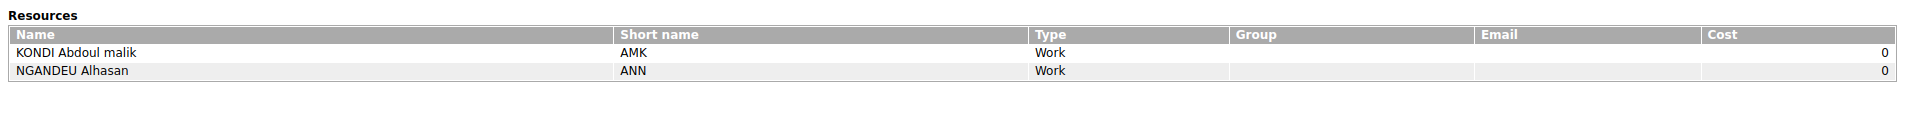
\includegraphics[height=3cm,width=16cm]{images/resources.png}
\section{Détails des événements passé pendant les cinq (5) jour}
\subsection{Jour 1 : Lundi}

\ La journée du lundi est la journée où nous avons rencontré le directeur général de Urbis foundation et nous avons longuement discuté sur les modalités du stage et nous avons également éclaircit certain point de divergence notamment nos convention. En effet après une longue discussion nous somme parvenu à nous comprendre et le directeur général de Urbis foundation nous a présenté notre maître de stage qui doit nous assister tout au long de notre stage ainsi que l’environnement dans lequel nous allons travailler. Après cette échange nous somme remonter vers notre institution au niveau de notre directeur pour lui faire par de la discussion entretenu entre nous stagiaire et le directeur général de Urbis foundation. 

\newpage
\subsection{Jour 2 : Mardi}
\ Le journée du mardi est la journée où nous avons pris place des les locaux qui nous ont été attribué. En effet après s’être installer nous avons sans plus tarder débuté l’analyse en recueillant des informations chez la bibliothécaire notamment les informations concernant le mode de fonctionnement de leur bibliothèque ainsi que toute ce qui serai nécessaire à faciliter notre analyse puis nous avons également débuté le diagramme des cas d’utilisation en nous basent sur toute les informations récoltées lors de notre analyse.\\
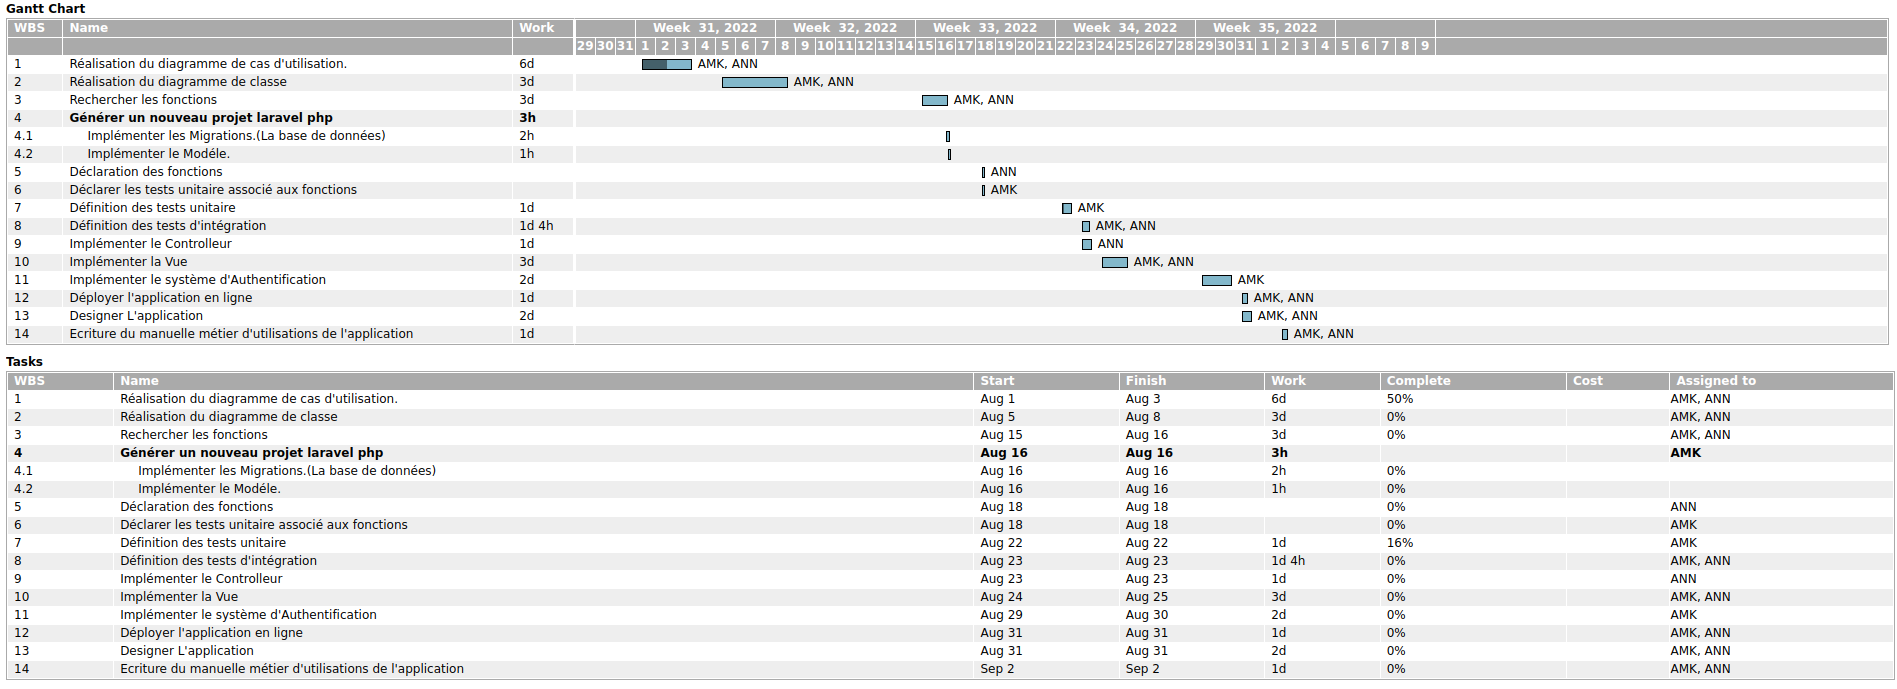
\includegraphics[height=15cm,width=22cm]{images/jour2.png}

\subsection{Jour 3 : Mercredi}
\ Le journée du mercredi est la journée où nous avons réussi à terminer notre diagramme de cas d’utilisation avec quelques derniers ajustement de ce dernier, ce qui nous a permis d’entamer le diagramme de classe métier qui a débuté avec une conception global puis nous avons usé des informations de notre diagramme de cas d’utilisation afin de déceler les informations clé pour une clarté de notre diagramme. Ainsi pour cette journée du mercredi nous avons réussi à faire cinquante pour cent de notre diagramme de classe.\\
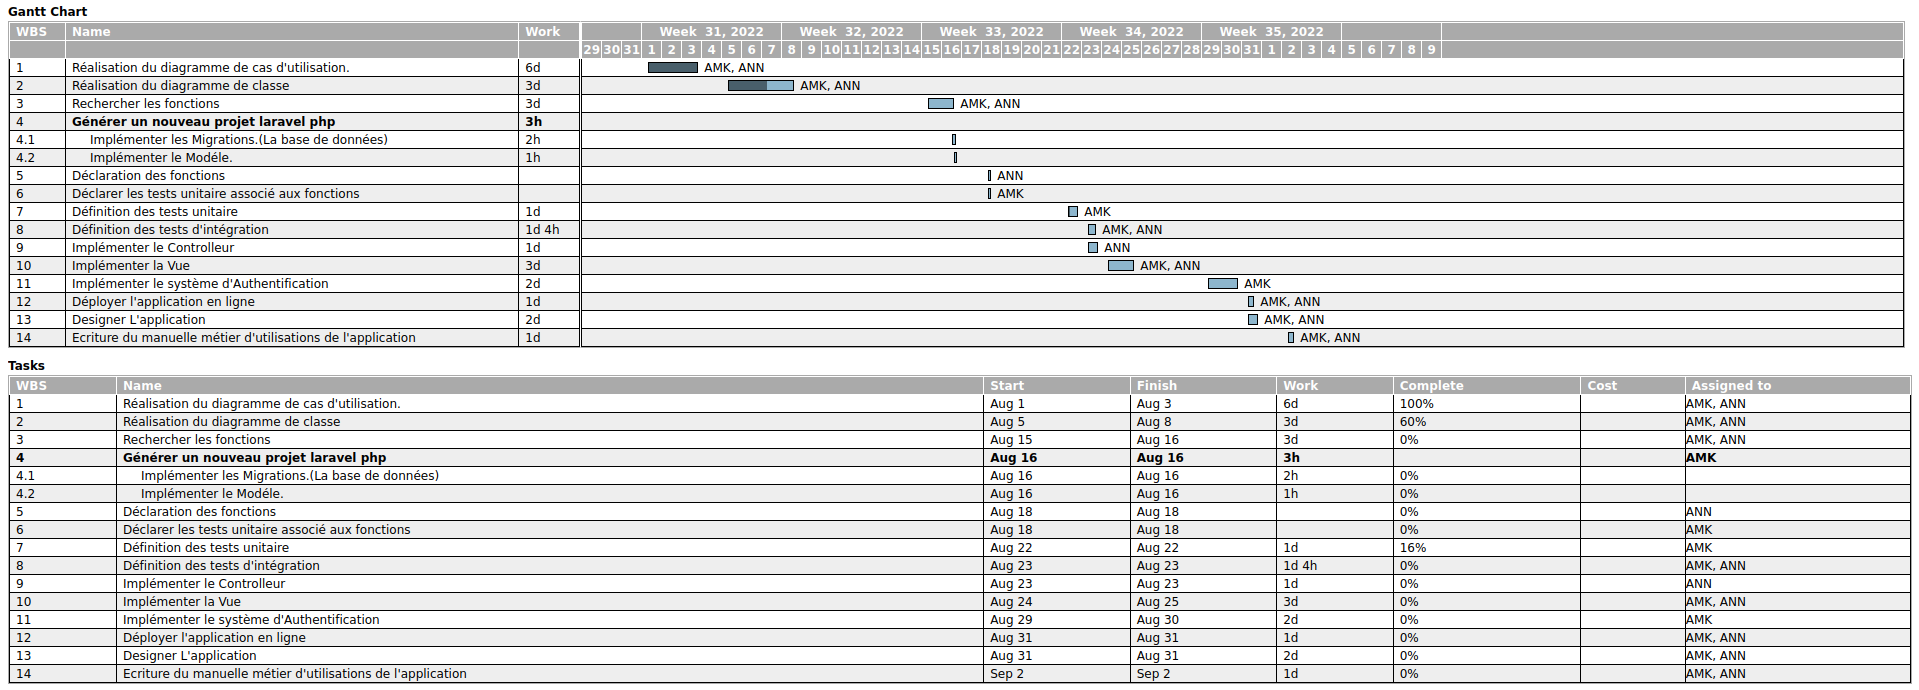
\includegraphics[height=15cm,width=22cm]{images/jour3.png}
\subsection{Jour 4 : Jeudi}
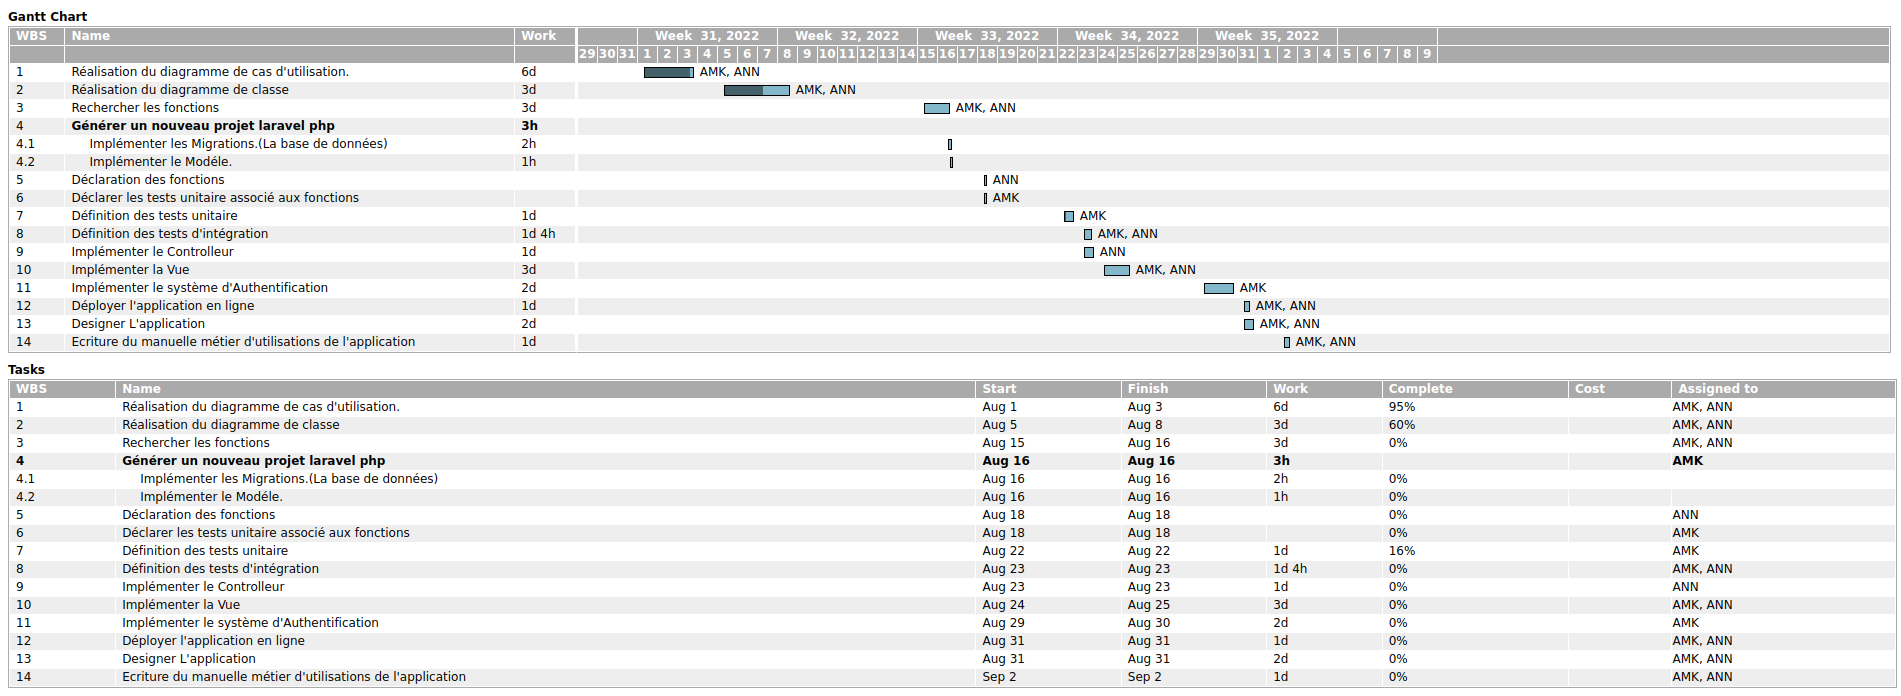
\includegraphics[height=15cm,width=22cm]{images/jour4.png}
Les activités fait le jeudi sont:
\begin{itemize}
\item Le début de la modélisation du diagramme de classe sous \textbf{modélio}.
\end{itemize}

\textbf{NB:}\\
Le jeudi soir nous n'avons pas pu travailler car malik était tombé malade.

\subsection{Jour 5 : Vendredi}
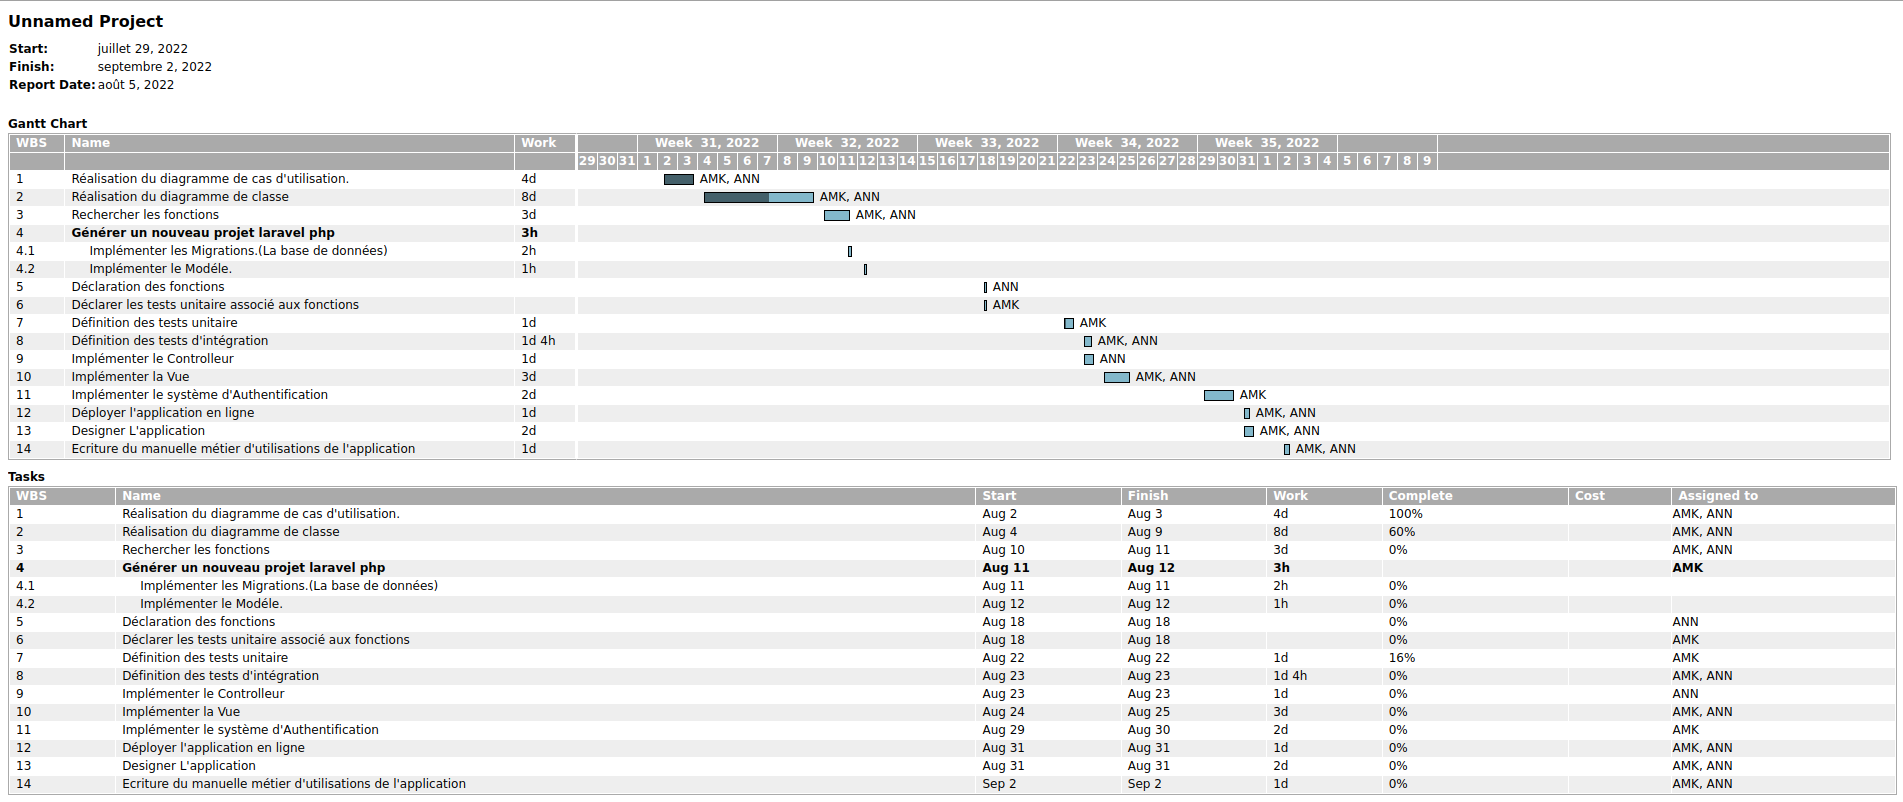
\includegraphics[height=15cm,width=22cm]{images/jour5.png}
Les activités fait ce vendredi ont été :
\begin{itemize}
\item La mise à jour de notre répertoire de travail sur git.
\item La mise à jour de notre diagramme de gant.
\item La consultation des registres de données chez la bibliothécaire.
\end{itemize}
\section{Conclusion}
	En résumé, cette semaine nous avons réalisé \textbf{75\%} du modèle.\\
	Le modèle était estimé à 10 jours (du 1 août au 12 août 2022 [\textit{prévision réel contrairement au gant affiché erreur technique}]). Mais aujourd'hui nous somme sûr que nous le ferrons en 7 jours (avant le 10 août 2022).

\end{document}




